\documentclass{article}
\usepackage[utf8]{inputenc}
\usepackage{tikz}
\usetikzlibrary{arrows}
\usepackage{pgf}
\usepackage{schemabloc} 

\title{LEPL1101 Problème P1}
\author{Groupe 34}
\date{Février 2020}

\begin{document}

\maketitle

\section{Introduction}

\section{Blocs fonctionnels}
    \subsection{Principe physique}
    
    \subsection{Emetteur}
        \begin{tiny}
        \begin{tikzpicture}
            \sbEntree{E}
            \sbBloc{entree}{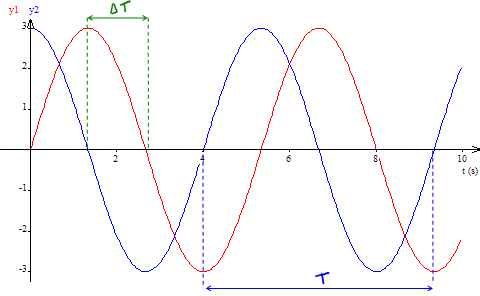
\includegraphics[scale=0.1]{imageTest.png}}{E}
            \sbRelier{E}{entree}
            
            \sbBloc{LC}{carré->sin}{entree}      
            \sbRelier[]{entree}{LC}
            \sbBloc{sin}{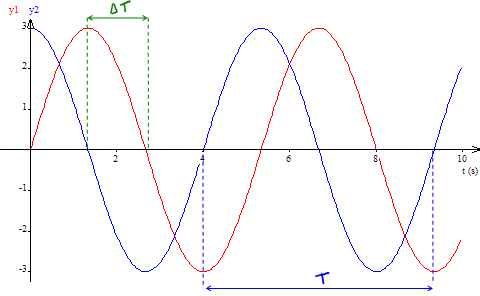
\includegraphics[scale=0.1]{imageTest.png}}{LC}
            \sbRelier[]{LC}{sin}
            
            \sbBloc{hp}{haut-parleur}{sin}
            \sbRelier[]{sin}{hp}
            \sbBloc{son}{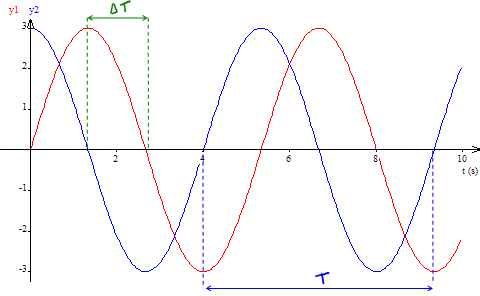
\includegraphics[scale=0.1]{imageTest.png}}{hp}
            \sbRelier[]{hp}{son}
            \sbSortie{S}{son}
        \end{tikzpicture}
        \end{tiny}
    
    \subsection{Récepteur}
        \begin{tiny}
        \begin{tikzpicture}
            
            \sbEntree{E}
            \sbBloc{entree}{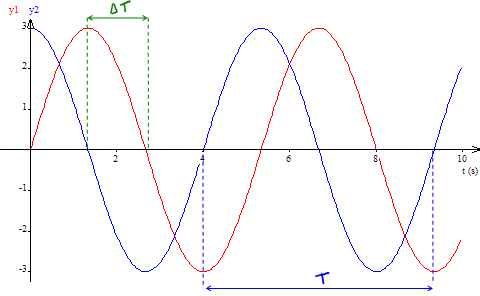
\includegraphics[scale=0.1]{imageTest.png}}{E} % input
            \sbRelier{E}{entree}
            
            \sbBloc{compA0}{Comp 1 et 2}{entree}      
            \sbRelier[]{entree}{compA0}
            \sbBloc{carre}{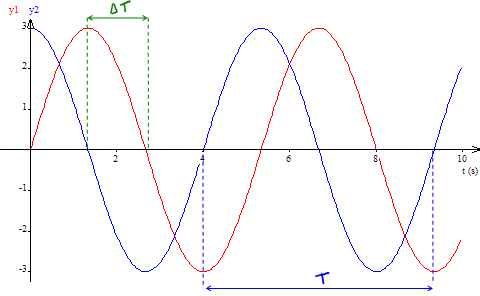
\includegraphics[scale=0.1]{imageTest.png}}{compA0} % carré
            \sbRelier[]{compA0}{carre}
            
            \sbBloc{compC1C2}{Comp 3}{carre}
            \sbRelier[]{carre}{compC1C2}
            \sbBloc{diff}{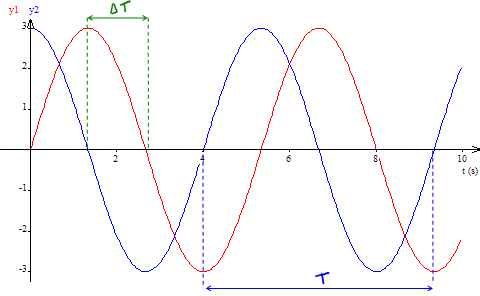
\includegraphics[scale=0.1]{imageTest.png}}{compC1C2}      %différence
            \sbRelier[]{compC1C2}{diff}
            
            	\sbDecaleNoeudy[4]{carre}{point1}
            \sbBloc{RC}{Dephasage de pi/2}{point1}
            \sbRelieryx{carre}{RC}
            \sbBloc{cond}{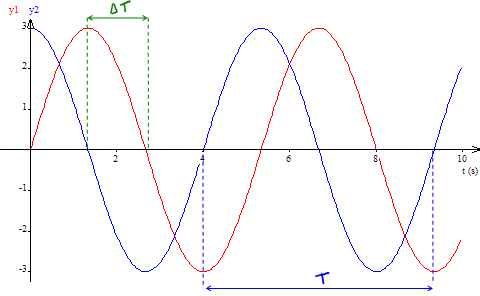
\includegraphics[scale=0.1]{imageTest.png}}{RC} % déphasé
            \sbRelier[]{RC}{cond}
            
            \sbBloc{condCheck}{Comp 4}{diff}
            \sbRelier[]{diff}{condCheck}
            \sbRelierxy[]{cond}{condCheck}
            	\sbDecaleNoeudx[5]{condCheck}{point21}
            	\sbDecaleNoeudy[10]{point21}{point22}
            	\draw[->] (condCheck) -- ++(1.5,0) -- ++(0,-2.6) -- ++(-0.7,0);
            \sbBlocr{resultAC}{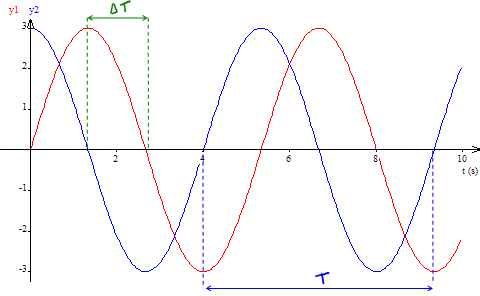
\includegraphics[scale=0.1]{imageTest.png}}{point22} % AC
            
            \sbBlocr{capa}{Effet capacitif}{resultAC}
            \sbRelier[]{resultAC}{capa}
            \sbBlocr{resultDC}{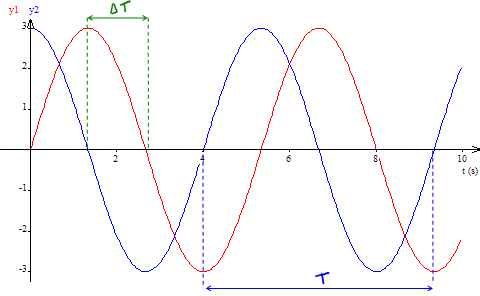
\includegraphics[scale=0.1]{imageTest.png}}{capa} % DC
            \sbRelier[]{capa}{resultDC}
            
        \end{tikzpicture}
        \end{tiny}
        
        ...
        
\section{Série de Fourrier et contenu spectral}
    \subsection{}
        
        

\end{document}
